\documentclass[11pt]{article}
\usepackage{graphicx}
\usepackage{float}
\usepackage{amsmath}
\usepackage{amsfonts}
\usepackage[brazilian]{babel}
\usepackage[utf8]{inputenc}
\usepackage[T1]{fontenc}

\begin{document}

\title{Matemática Elementar: Conjuntos numéricos}
\author{Erik Perillo}
\date{}
\maketitle
\begin{abstract}
Nesta etapa, falaremos sobre os tipos de números que podemos encontrar por aí
na aventura da matemática.
\end{abstract}

\newpage

\tableofcontents

\newpage

\section{Conjuntos Numéricos}
No nosso dia a dia, nós vivemos classificando as coisas. Classificamos, por
exemplo, comidas em diferentes tipos. Temos as frutas, os legumes, as carnes 
etc. Por que fazemos isso? Ora, porque cada um desses tipos de alimentos tem
características bem únicas deles, e é útil separá-los. 
Frutas são em geral doces, carnes em geral se deve cozinhar antes de comer. 
Sabemos que misturar frutas em uma salada de frutas é uma boa ideia, mas 
misturar carnes e frutas em uma mesma coisa quase nunca dá certo!
\paragraph{}
Como matemáticos também são humanos, eles fizeram a mesma coisa com números.
Ao longo do tempo, foi-se percebendo que os números são diferentes, e alguns
deles têm características bem especiais, de um modo que faria sentido separá-los
em classes distintas. Foi dessa ideia que foram desenvolvidos os
\textit{conjuntos numéricos}. Os conjuntos numéricos colocam uma ordem nos 
números e nos permitem analisar as características deles, de forma que fica
mais fácil saber o que podemos e o que não podemos fazer com os números!
\paragraph{}
Nas próximas seções, então, vamos aprender mais sobre esses números.

\subsection{Números Naturais}
\paragraph{}
No começo, a gente só sabia contar ovelhas. O pastor só precisava saber quantas
ovelhinhas ele tinha: se eram 1, 5, 10 ou até mesmo nenhuma (0). 
\paragraph{}
O mínimo que ele podia ter era nenhuma ovelha, ou seja, 0 ovelhas. Faz sentido
eu ter $-2$ ovelhas? Essa ideia não era muito bem vista ainda, então isso não
existia naquela época. Eu posso ter meia ovelha? Se estiver viva, não, então
não fazia sentido também pensar em coisas como o número $0.5$. Fica claro, 
então, que só se precisava de números \emph{inteiros} e \emph{positivos}.
É daí, então, que surgem os números \textbf{naturais}, que são representados
pelo símbolo $\mathbb{N}$. Os números naturais são:
$$0, 1, 2, 3, \dots$$
E assim vão até o infinito.

\subsection{Números Inteiros}
\paragraph{}
Depois de muito contar ovelhinhas, a gente começou a ser ganancioso e lidar com
dinheiro. Agora se podia comprar e vender ovelhinhas. Com isso, naturalmente,
começaram a aparecer dívidas. Muita gente começou a dever moedinhas e a gente
precisava manter isso documentado. Mas como a gente representaria que estamos
devendo 3 moedinhas? Foi daí que começou a aparecer o conceito de o que é um
\emph{número negativo}. A gente ainda não pensava em coisas como meias moedas,
então só começamos pensando na falta de coisas inteiras, como moedas.
\paragraph{}
Foi daí, então, que surgiram os números \textbf{inteiros}, representados pelo
símbolo $\mathbb{Z}$. Os números inteiros são só uma extensão dos números 
naturais, adicionando o \emph{negativo} deles:
$$\dots, -5, -4, -3, -2, -1, 0, 1, 2, 3, 4, 5 \dots$$
E assim vai, desde o infinito negativo até o infinito positivo.
\paragraph{}
Quando eu digo que os inteiros são só uma extensão dos naturais, eu não estou
exagerando! Percebeu como os inteiros têm todos os números naturais possíveis?
Então ele realmente é uma extensão. Podemos dizer, então, que \textbf{todo
número natural também é um número inteiro}. Por exemplo, o 3 é inteiro e também
é natural. Não dá pra dizer o contrário, porém. Nem todo número inteiro é 
natural. O $-3$, por exemplo, é inteiro, mas não é natural. 
\paragraph{}
A gente pode, então, dizer que os naturais estão \textbf{contidos} nos inteiros.
Dá pra representar isso pelo desenho:
\begin{figure}[H]
  		\centering
    	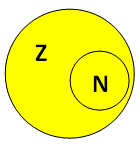
\includegraphics[width=0.3\textwidth]{imgs/n_z.png}
		\caption[9pt]{Números naturais estão dentro dos inteiros}
\end{figure}

\subsection{Números Racionais}
\paragraph{}
Chegou uma hora que os cachaceiros começaram a mexer com matemática. A partir
desse momento, era importante saber contar, por exemplo, quanto custava meia
garrafa de pinga, ou seja, uma \textbf{fração} da garrafa. 
Como representar isso então? Surgiu daí a necessidade de inventar números para
isso. No caso de meia garrafa, precisamos então de algo como $\frac{1}{2}$.
Esse número certamente é diferente dos que existiam antes: Ele 
\textbf{não é inteiro}, porque meia garrafa de pinga certamente não é uma 
garrafa inteira. 
\paragraph{}
Surgiu então a necessidade de classificá-los como outra classe de número, e 
então apareceu o conceito de números \textbf{racionais}, representados pelo
símbolo \textbf{Q}. Entre eles, estão os números:
$$-\frac{2}{5}, \; \frac{1}{3}, \; \frac{23}{54}, \; \dots$$
Ou seja, todo número que você representa como uma fração. 
\paragraph{}
Dá também pra escrevê-los na forma de números decimais. $\frac{1}{2}$, 
por exemplo, também é $0.5$, mas não é porque escrevemos dessa forma que 
o $0.5$ deixa de ser racional. Alguns racionais, quando representados desse
jeito, ficam bem estranhos. Por exemplo: o $\frac{1}{3}$, quando representado
na forma decimal, fica:
$$0.33333333333 \dots$$
Esses 3 acabam? Não! Nunquinha! Isso certamente é um número muito estranho, mas
ainda é racional, porque ele \textbf{tem uma representação como uma fração}.
\paragraph{}
M-mas e os números
inteiros? São racionais também? Pra responder isso, temos que responder: 
Conseguimos representar um inteiro como uma fração? A resposta é: 
claro que sim! Pegue o número 4, por exemplo. Pra escrevê-lo como uma fração,
podemos simplesmente escrevê-lo como $\frac{4}{1}$. Fácil, não? Então este é
o fato: \textbf{todo número inteiro é também racional}. Do mesmo jeito que os
naturais estão dentro dos inteiros, os inteiros estão dentro dos racionais.
Podemos representá-los desta maneira:
\begin{figure}[H]
	\centering
	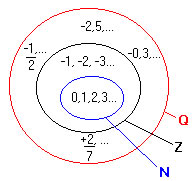
\includegraphics[width=0.35\textwidth]{imgs/n_z_q.jpg}
	\caption[9pt]{Números racionais engolem os inteiros}
\end{figure}

\subsection{Números Irracionais}
\paragraph{}
Parece que com os naturais, inteiros e racionais, já da pra formar todos os 
números que se possa imaginar, né? Infelizmente, não é assim. Tem alguns 
números que, pasme: não são inteiros, e nem dá pra representar usando uma
fração! Isso é muito estranho, mas é a verdade. Pegue, por exemplo, o número
$\sqrt{2}$. Você consegue representá-lo como uma fração? Nem perca seu tempo,
porque já foi provado matematicamente que não. Logicamente, então, temos
que criar uma nova classe para números assim. Eles então são os números 
\textbf{irracionais}. Todo número que 
\textbf{não pode ser representado como uma fração} é irracional. 
Ele é representado pelo símbolo $\mathbb{I}$.
Outros números como $\pi$ também foram provados ser irracionais. 
\paragraph{}
Os números irracionais, diferente dos que nós vimos até agora, não englobam os
outros. Os inteiros não estão contidos nos irracionais, por exemplo. Então, no
desenho que estamos fazendo, eles ficam assim:
\begin{figure}[H]
	\centering
	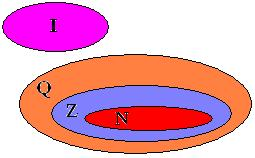
\includegraphics[width=0.4\textwidth]{imgs/n_z_q_i.jpg}
	\caption[9pt]{Números irracionais não contém os outros}
\end{figure}

\subsection{Números Reais}
\paragraph{}
Os números \textbf{reais}, representados por $\mathbb{R}$, não são nada em 
especial. Eles são apenas a \textbf{união dos racionais com os irracionais}. 
É como se você pegasse um saco, jogasse todos os números racionais, todos os
irracionais lá dentro, e dissesse: ``Tudo isso aqui são números reais.''
\paragraph{}
Qualquer número, então, é um número real. Daí vem seu nome: real. Qualquer 
número que existe na realidade é real. Nosso diagrama, cada vez mais completo,
fica assim, então:
\begin{figure}[H]
	\centering
	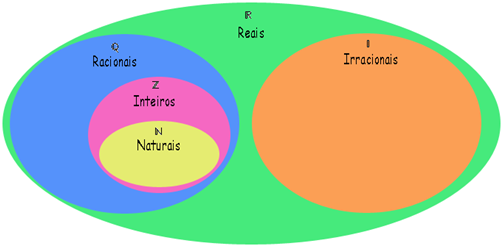
\includegraphics[width=0.7\textwidth]{imgs/n_z_q_i_r.png}
	\caption[9pt]{Qualquer número que existe na natureza é real}
\end{figure}

\subsection{Números Complexos}
\paragraph{}
Só para você saber, existem outros tipos de números que são chamados de 
complexos. A gente não vai falar sobre eles agora, mas saiba que eles existem.

\newpage


\section{Outros Conjuntos}
\subsection{Conjuntos personalizados}
\paragraph{}
Além dos conjuntos que nós vimos, nós podemos criar conjuntos. Podemos, por 
exemplo, só querer saber dos números pares de 2 a 8. Podemos, então, criar um
conjunto $A$:
$$A = \{2, \; 4, \; 6, \; 8\}$$
E é dessa forma que se escreve.

\subsection{Intervalos fechados}
\paragraph{}
Na subseção acima, usamos um conjunto pequeno. E se quiséssemos representar um
conjunto bem grande? Escreveríamos um a um? Claro que não. Podemos então
representar os conjuntos como $[x, y]$. Isso se chama um \textbf{intervalo}.
Os números $1,2,3\dots$ até 98, por exemplo, ficaria:
$$[1, \; 98]$$
Isso é um intervalo \textbf{fechado}, ou seja, os números nos extremos estão
incluidos no intervalo.

\subsection{Intervalos abertos}
\paragraph{}
Os intervalos abertos são parecidos com os fechados, mas os números do extremo
não são incluídos. Para eles, usa-se um parênteses normal. Por exemplo, se 
queremos representar os números de 1 a 96, sem contar o 1 e o 96, escrevemos:
$$(1, \; 96) = 2, \; 3, \; \dots \; , 95$$
Você pode misturar as coisas. Um intervalo pode ser fechado de um lado e 
aberto do outro, tanto faz os lados. Por exemplo: os números de 1 a 96 sem 
contar só o 96 ficam $[1, \; 96)$.

\newpage

\section{Símbolos para Conjuntos}
\paragraph{}
Na seção passada, falamos bastante sobre um conjunto \textbf{conter} o outro.
Frases do tipo são o tempo todo usadas em matemática, então eles criaram 
símbolos que significam essas frases. Alguns símbolos são:

\begin{itemize}
	\item $\subseteq$ -- Está contido em. Exemplo:
	      \paragraph{}
		  Os naturais \textbf{estão contidos} nos inteiros 
		  $\implies \mathbb{N} \subseteq \mathbb{Z}$

	\item $\not\subseteq$ -- \textbf{Não} está contido em. Exemplo:
	      \paragraph{}
		  Os inteiros \textbf{não estão contidos} nos naturais 
		  $\implies \mathbb{Z} \not\subseteq \mathbb{N}$

	\item $\supseteq$ -- Contém. Exemplo:
	      \paragraph{}
		  Os inteiros \textbf{contêm} os naturais
		  $\implies \mathbb{Z} \supseteq \mathbb{N}$

	\item $\not\supseteq$ -- \textbf{Não} contém. Exemplo:
	      \paragraph{}
		  Os inteiros \textbf{não contêm} os reais
		  $\implies \mathbb{Z} \not\supseteq \mathbb{R}$

	\item $\in$ -- Pertence a. Exemplo: 
		  \paragraph{}
		   O número 3 \textbf{pertence a}os naturais 
		   $\implies 3 \in \mathbb{N}$
	
	\item $\not\in$ -- \textbf{Não} pertence a. Exemplo: 
		  \paragraph{}
		   O número $\pi$ \textbf{não pertence a}os racionais 
		   $\implies \pi \in \mathbb{R}$
\end{itemize}
\paragraph{}
Note que os símbolos que lembram uma letra C (ex. $\subseteq$) são usados
apenas em conjuntos. É como se falássemos de bolsas: uma bolsa está contida
em outra. Não faz sentido escrever, por exemplo, $3 \subseteq \mathbb{R}$.
Por que não? Porque o 3 é um \textbf{elemento}, e não um conjunto. Ele é um
lápis, e não uma bolsa. Quando falamos sobre um elemento estar em um conjunto,
usamos o $\in$.

\section{Exercícios}
\begin{enumerate}
	\item Escreva a que conjunto pertence cada um dos números abaixo.
	\begin{enumerate}
		\item $-3$
		\item $0$
		\item $23$
		\item $0.5$
		\item $\frac{3}{4}$
		\item $\pi$
		\item $-\frac{1}{3}$
	\end{enumerate}

	\item Escreva os números que os intervalos a seguir contêm. Exemplo:
		  $$[1,3] = 1,2,3$$
	\begin{enumerate}
		\item $[4,8]$
		\item $[-2,3]$
		\item $[-3,-1]$
		\item $(1,6)$
		\item $(-1,6)$
		\item $(1,7]$
		\item $[0,4)$
	\end{enumerate}

	\item Assinale as alternativas como verdadeiro ou falso.
	\begin{enumerate}
		\item $\mathbb{Z} \subseteq \mathbb{R}$
		\item $3 \subseteq \mathbb{Z}$
		\item $\mathbb{N} \subseteq \mathbb{Z}$
		\item $\frac{1}{2} \in \mathbb{Q}$
		\item $\pi \not\in \mathbb{R}$
	\end{enumerate}
\end{enumerate}

\newpage

\section{Respostas aos Exercícios}
\begin{enumerate}
	\item
	\begin{enumerate}
		\item Inteiros $(\mathbb{Z})$
		\item Naturais $(\mathbb{N}$
		\item Naturais $(\mathbb{N}$
		\item Racionais $(\mathbb{Q}$
		\item Racionais $(\mathbb{Q}$
		\item Irracionais $(\mathbb{I}$
		\item Racionais $(\mathbb{Q}$
	\end{enumerate}

	\item
		  $$[1,3] = 1,2,3$$
	\begin{enumerate}
		\item $\{4,5,6,7,8\}$
		\item $\{-2,-1,0,1,2,3\}$
		\item $\{-3,-2,-1\}$
		\item $\{2,3,4,5\}$
		\item $\{0,1,2,3,4,5\}$
		\item $\{2,3,4,5,6,7\}$
		\item $\{0,1,2,3\}$
	\end{enumerate}

	\item 
	\begin{enumerate}
		\item Verdadeiro.
		\item Falso. (Não se compara elementos com conjuntos com esse operador)
		\item Verdadeiro.
		\item Verdadeiro.
		\item Falso.
	\end{enumerate}
\end{enumerate}


\end{document}
